%Ivan Iotzov and Lucas Parra submission to CCN 2019, Berlin

\documentclass[10pt,letterpaper]{article}

\usepackage{ccn}
\usepackage{pslatex}
\usepackage{apacite}
\usepackage{graphicx}

\graphicspath{ {./figures/} }


\title{Using EEG to Predict Speech Intelligibility}
 
\author{{\large \bf Ivan Iotzov (iiotzov@gradcenter.cuny.edu)} \\
  Department of Biomedical Engineering, 160 Convent Avenue\\
New York, NY 10030, U.S.A.
  \AND {\large \bf Lucas C. Parra (parra@ccny.cuny.edu)} \\
  Department of Biomedical Engineering, 160 Convent Avenue\\
New York, NY 10030, U.S.A.}


\begin{document}

\maketitle


\section{Abstract}
{
\bf
Speech signals have the ability to entrain brain activity to the rapid 
fluctuations found in speech sounds. This entrainment can be measured 
using electroencephalographic (EEG) recordings and is strong enough to allow 
discrimination between attended and unattended speech sources. In this study,
we investigated whether these entrainment responses can be used to measure 
how intelligible a speech signal is to a subject. We hypothesized that when 
intelligibility is degraded, attention wanes and the stimulus-response 
correlation will decrease. To test this, we measured a listener's ability 
to detect words in noisy, natural speech while recording brain activity using 
EEG. We altered intelligibility by presenting congruent or incongruent video 
of the speaker along with their speech. For almost all subjects, word 
detection performance improved in the congruent condition and this improvement 
coincided with an increase in stimulus-response correlation. We conclude that 
simultaneous recordings of perceived sound and EEG activity may represent a 
practical tool to assess speech intelligibility, specifically in the context 
of hearing aid devices.
}

\begin{quote}
\small
\textbf{Keywords:} 
EEG; stimulus-response correlation; 
speech comprehension; speech intelligibility
\end{quote}

\section{Introduction}

While listening to sounds, brain activity follows the fast fluctuations of 
the acoustic stimulus \cite{Ding2014a,Haegens2018}. This effect can also
be observed in subjects listening to speech signals, 
where EEG and MEG signals have been shown to correlate 
with fluctuations in signal amplitude and spectral content 
\cite{Luo2007,Horton2014}. This stimulus-driven brain activity has been linked
to attention \cite{ZionGolumbic2013,OSullivan2015}, in particular in 
multi-speaker scenarios where these correlations are thought to reflect 
the listener's ability to follow the attended speech stream. We attribute this
speech tracking phenomenon to an exogenous stimulus-driven process due to the 
consistent responses elicited by a speech stimulus across subjects 
\cite{Ki2016,Cohen2017}. 

For noisy speech, correlations can still be found between the brain response 
and the amplitude envelope of the clean speech \cite{Ding2013,Vanthornhout2017}.
This may be a reflection of the incredibly robust ability of listeners to 
understand speech despite significant noise or distortions. A consistent 
confound in previous research has been that speech intelligibility is 
modulated by altering various properties of the stimulus. Because of this,
it is difficult to determine whether changes in speech tracking are 
caused by genuine changes in auditory processing or merely a reflection of the
altered stimulus. We have attempted to mitigate this confound by keeping 
the stimulus unchanged and modulating speech intelligibility through 
visual cues. The audio presented to subjects in our two experimental conditions
is identical and we modulate intelligibility by presenting visuals that 
are either congruent (i.e. the mouth of the speaker and the heard audio align)
or incongruent (i.e. heard audio and speaker do not align).



\section{Methods}

\subsection{Stimulus Presentation and Behavioral Measures}

  The stimuli used in this experiment were previously used in other 
  speech tracking experiments with EEG \cite{Crosse2015,Crosse2016}.
  The stimuli consist of 30 audiovisual talking head clips of President
  Barack Obama discussing the Affordable Care Act, each 60s long. In total, 
  there were four stimulus conditions combining -9 dB/ -6 dB noise and 
  congruent/incongruent visuals in a 2 x 2 design. Subjects were presented
  with all 30 stimuli in each of the four conditions, for a total of 120
  trials that took place over 2 experimental sessions. The sessions were
  seperated by at least one week to minimize the effects of subject 
  memory on the results.

  Before each 60s trial, subjects were presented with a `target word' and 
  were instructed to press a button whenever they heard the target. Target 
  words were selected so that each word occurs the same number of times
  in all four conditions. Responses within 1.5s of word presentation 
  were coded as correct detection and any responses outside of this window
  were coded as false alarms. Correct detections can be reported either 
  relative to the total number of target words (detection) or relative 
  to the total number of responses (precision). In order to capture 
  both of these properties, we report behavioral performance using the 
  F1 score, which is the harmonic mean of detection and precision.
  

\subsection{EEG and Stimulus Processing}

  EEG was recorded using a BioSemi Active II amplifier with 64 electrodes 
  arranged according to the International 10-20 system, in addition to 6
  electrooculogram (EOG) electrodes. The EEG was sampled at 512 Hz and 
  later downsampled to the framerate of the video presentation (30 Hz).
  Before correlation to the stimulus, the EEG signal was preprocessed as 
  follows: the initial value was subtracted from the data to remove the 
  DC offset. A high-pass 5th order Butterworth filter with a cutoff of 
  0.5 Hz was applied. The signal from the 6 EOG electrodes was regressed 
  out using a least-squares algorithm. Finally, artifacts and channels 
  with recording quality issues were removed.

  The steps used to calculate the stimulus amplitude envelope are as follows:
  the sound amplitude envelope is calculated as the absolute value of the 
  analytic signal after a Hilbert transform fo the raw mono sound signal 
  at its original sampling rate of 48 kHz. The result is then downsampled
  to the framerate of the video (30 Hz) and z-scored. Then, a Toeplitz matrix
  with 30 columns is constructed to capture up to a 1s delay.
  
\subsection{Stimulus-Response Correlation (SRC)}

  The models used in these types of analyses are typically encoding or 
  decoding models. The encoding approach uses various features of the 
  stimulus to predict the brain response. The decoding approach is the reverse,
  using the brain response to reconstruct the stimulus. Here, we used a 
  hybrid encoding and decoding approach \cite{Dmochowski2017}. The model 
  attempts to maximize the correlation between the encoded stimulus 
  $\hat{u}(t)$ and the decoded response $\hat{v}(t)$. The two signals 
  are defined as:
  
    $$\hat{u}(t) = h(t) * s(t)$$
    $$\hat{v}(t) = \sum_{i} w_ir_i(t)$$
  where $s(t)$ is the sound amplitude envelope at time $t$, $h(t)$ is the 
  encoding filter applied to the stimulus signal, * represents convolution, 
  $w_i$ are the weights applied to the neural response, and $r_i(t)$ is the 
  EEG signal value at time $t$ at electrode $i$. The model parameters 
  $h(t)$ and $w_i$ are found using canonical correlation analysis (CCA).
  CCA looks to maximize the correlation between the encoded stimulus and the 
  decoded brain response by computing several components that each capture
  some portion of the correlated signal. The stimulus-response correlation (SRC)
  that we report is the sum of the correlation of $\hat{u}(t)$ and $\hat{v}(t)$
  for the first three components. For a full discussion of the method for 
  computing the spatial and temporal response functions, please see 
  \cite{Dmochowski2017}.

  The hybrid model is trained using data from all subjects in all conditions. 
  The resulting spatial and temporal response functions can be seen in 
  \ref{behavior}. The model is then used to separately compute SRC for each 
  subject in each of the four conditions.
  

% \subsection{Figures}

% Make sure that the artwork can be printed well (e.g. dark colors) and that 
% the figures make understanding the paper easy.
%  Number figures sequentially, placing the figure
% number and caption, in 10~point, after the figure with one line space
% above the caption and one line space below it, as in
% Figure~\ref{sample-figure}. If necessary, leave extra white space at
% the bottom of the page to avoid splitting the figure and figure
% caption. You may float figures to the top or bottom of a column, or
% set wide figures across both columns.

% \begin{figure}[ht]
% \begin{center}
% \fbox{CCN figure}
% \end{center}
% \caption{This is a figure.} 
% \label{sample-figure}
% \end{figure}

\begin{figure}[]
  \begin{center}
    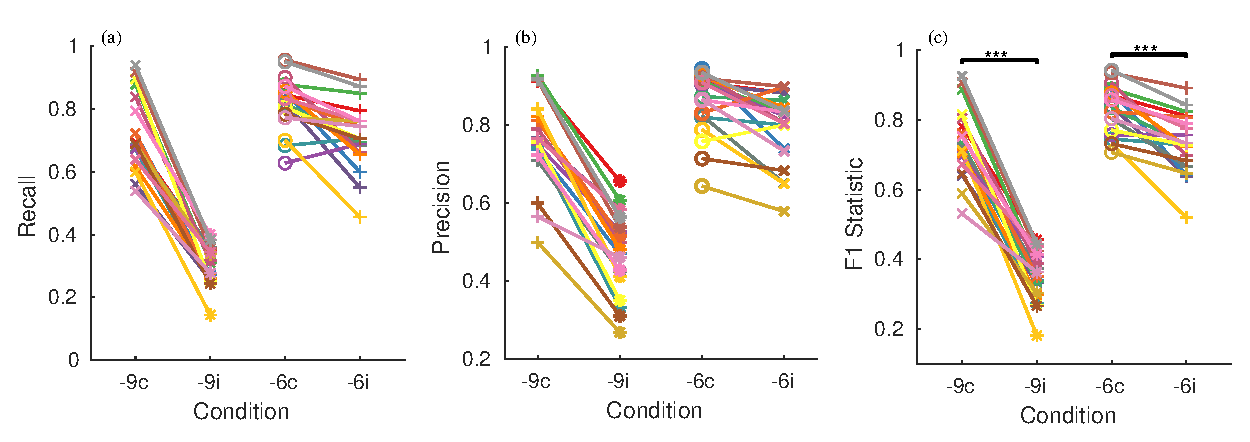
\includegraphics[width=\columnwidth]{Figure2}
  \end{center}
  \caption{}
  \label{behavior}
\end{figure}


\section{Results}

  \subsection{Congruent Visual Speech Increases Word Detection}

  \subsection{Congruent Visual Speech Increases Stimulus-Response Correlation}


\section{Conclusion}

conclusion here


\bibliographystyle{apacite}

\setlength{\bibleftmargin}{.125in}
\setlength{\bibindent}{-\bibleftmargin}

\bibliography{IotzovParraCCNSubmission2019}


\end{document}
